\chapter{Results and Evaluation}
\label{sec:results_and_evaluation}

\section{Simulation Result}

This simulation tested how the architecture works on the  test bench. The scheduler is connected to four clients and two servers in this test scenario. 


\begin{figure}[htb]
	\centering
	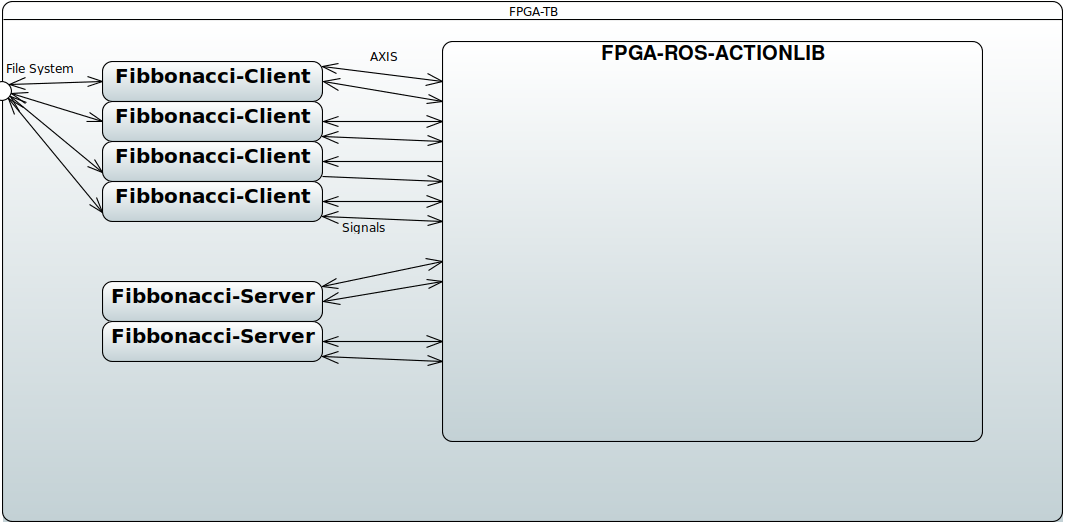
\includegraphics[width=.9\linewidth]{figures/fpga-tb2.png}
	\caption{Test Bench Architecture}
	\label{fig:hwfra-tbio}
\end{figure}

The Clients reads file from its hosting pc and read the content. Then it generates goals and send them out. After that, clients will waiting for the result and write it to a output file.

\begin{figure}[htb]
	\centering
	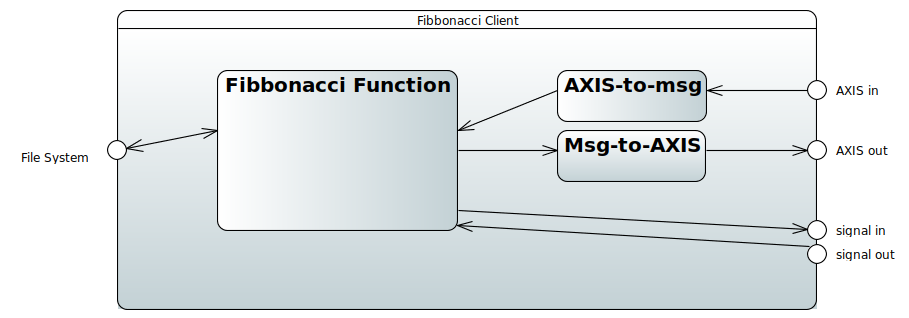
\includegraphics[width=.9\linewidth]{figures/fp-cli.png}
	\caption{Test Bench Client}
	\label{fig:client-general}
\end{figure}

\gls{hwfra} will listen all the clients and servers. If they are ready, then the architecture will link the chosen client and the chosen server together. 

Servers wait for goals from the input AXIS Stream after a success receive, it will return the $n^{th}$ number of the Fibonacci sequence.
\begin{table}[htb]
	\centering
	\caption{Example for the Input and Output}
	\begin{tabular}{l c c}
		\toprule
		Client Number  & Input  & Output\\ \midrule
        4	Servers	&	4	Clients	&	116	\\
        4	Servers	&	8	Clients	&	168	\\
        4	Servers	&	16	Clients	&	268	\\
        4	Servers	&	32	Clients	&	464	\\
        4	Servers	&	64	Clients	&	860	\\
        4	Servers	&	128	Clients	&	1642	\\
        4	Servers	&	256	Clients	&	3188	\\
		\bottomrule
	\end{tabular}
	\label{tab:sim-io}
\end{table}
After the last bit of result is transmitted, the Server will set it self to succeed state, and be ready for next goal. 

The overall process is showed in a following image. Indicating the general look of the entire process.

\begin{figure}[htb]
	\centering
	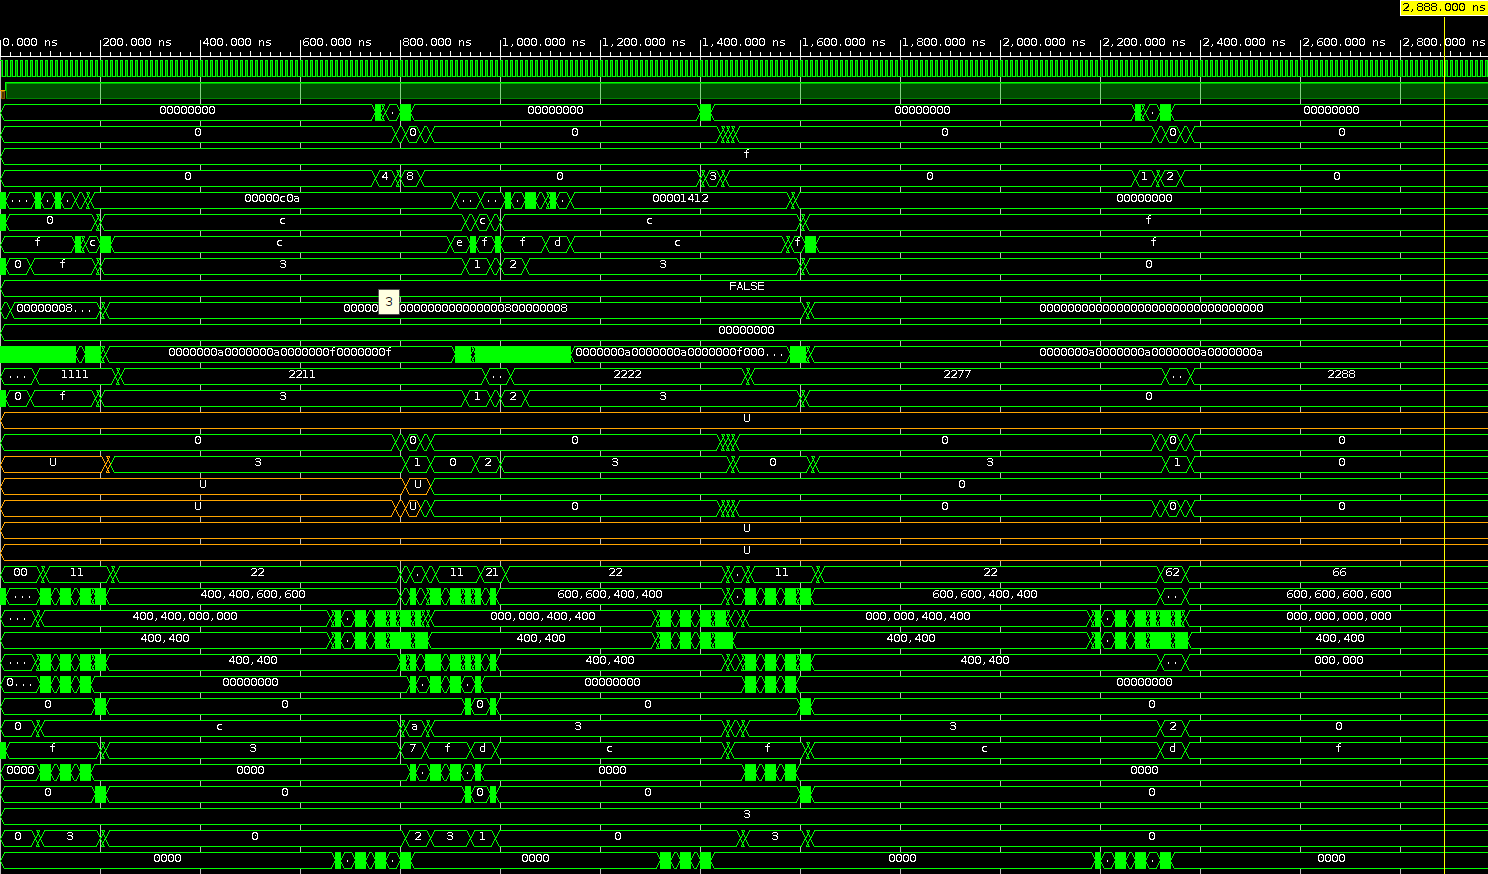
\includegraphics[width=.7\linewidth]{figures/sim.png}
	\caption{Simulation Result on 20ns}
	\label{fig:sim-overall}
\end{figure}


\subsection{Process Explanation}

This is the running log for the test bench process.

Before 70ns, all clients reading its input data via an AXIS Stream interface. Here is process is simulated by reading a file from the hosting operating system.

70ns:     All client finish reading their data head 

\begin{figure}[htb]
	\centering
	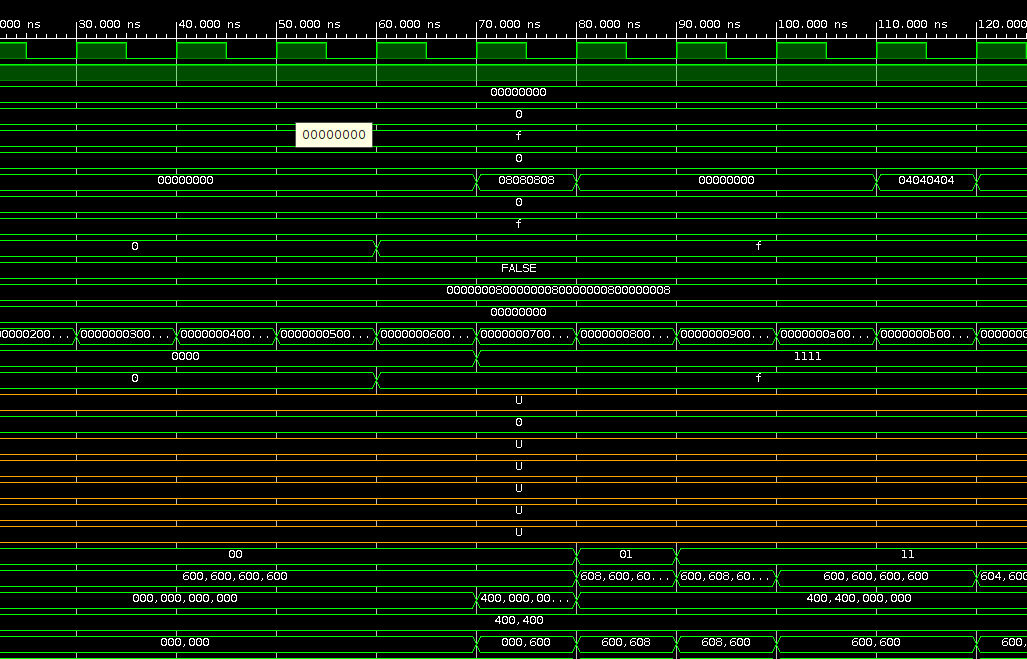
\includegraphics[width=.7\linewidth]{figures/new-sim/sim-20ns.png}
	\caption{Simulation Result on 20ns}
	\label{fig:sim-20}
\end{figure}

\newpage
80ns:     Server 1 linked to Client 3, data transport start ,server state set to 1 

90ns:     Server 2 linked to Client 2 

200ns:    Last bit of the data Client 3 and Client 2 , server validating data 

\begin{figure}[htb]
	\centering
	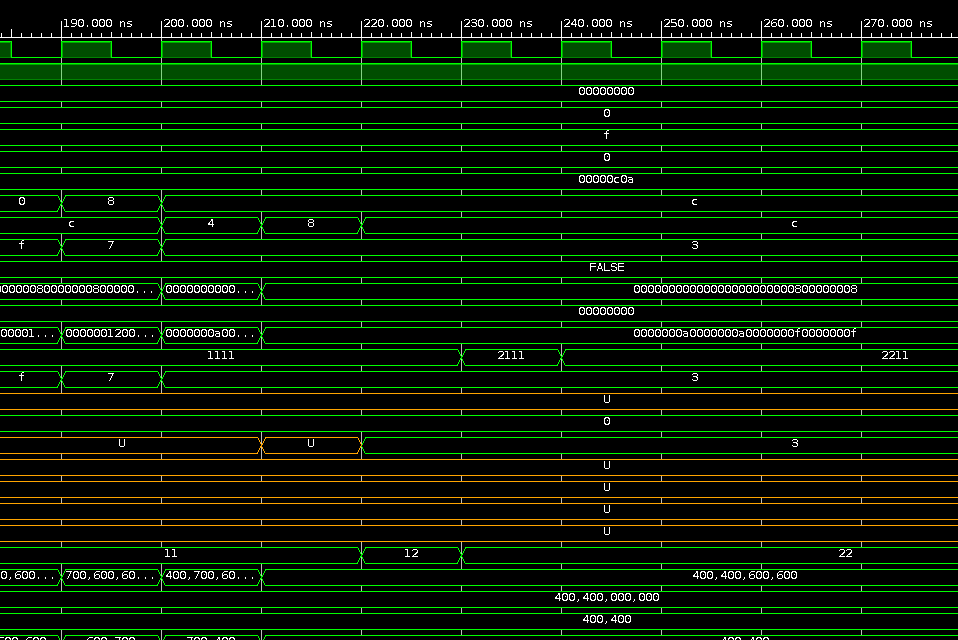
\includegraphics[width=.7\linewidth]{figures/new-sim/sim-190ns.png}
	\caption{Simulation Result on 190ns}
	\label{fig:sim-190}
\end{figure}

\newpage
220ns:    Data verified Server 1 send accept state set to ACTIVE 

230ns:    Data verified Server 0 send accept state set to ACTIVE ,  Client 3 set state to ACTIVE

240ns:    Client 2 set state to ACTIVE

\begin{figure}[htb]
	\centering
	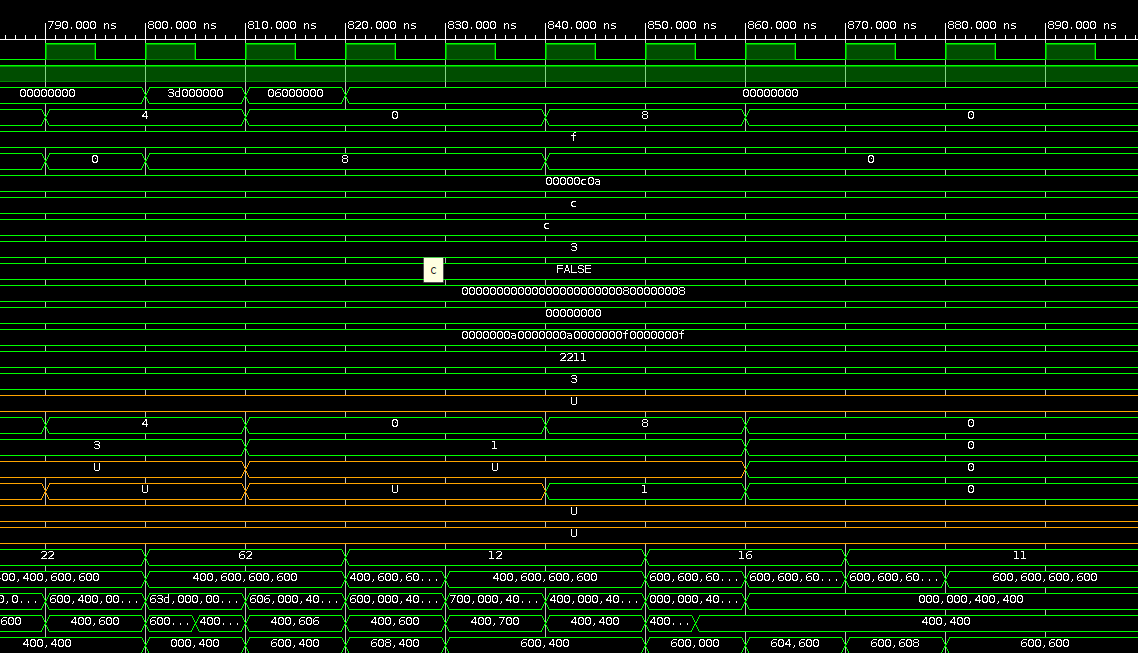
\includegraphics[width=.7\linewidth]{figures/new-sim/sim-780ns.png}
	\caption{Simulation Result on 780ns}
	\label{fig:sim-780}
\end{figure}

\newpage
800ns:    Server 1 state set to SUCCEED after complete the computation send the last bit of result.

820ns:    Server 1 state set to ready and receiving data from Client 1

850ns:    Server 0 state set to SUCCEED after complete the computation send the last bit of result.

870ns:	  Server 0 state set to ready and receiving data from Client 1

\begin{figure}[htb]
	\centering
	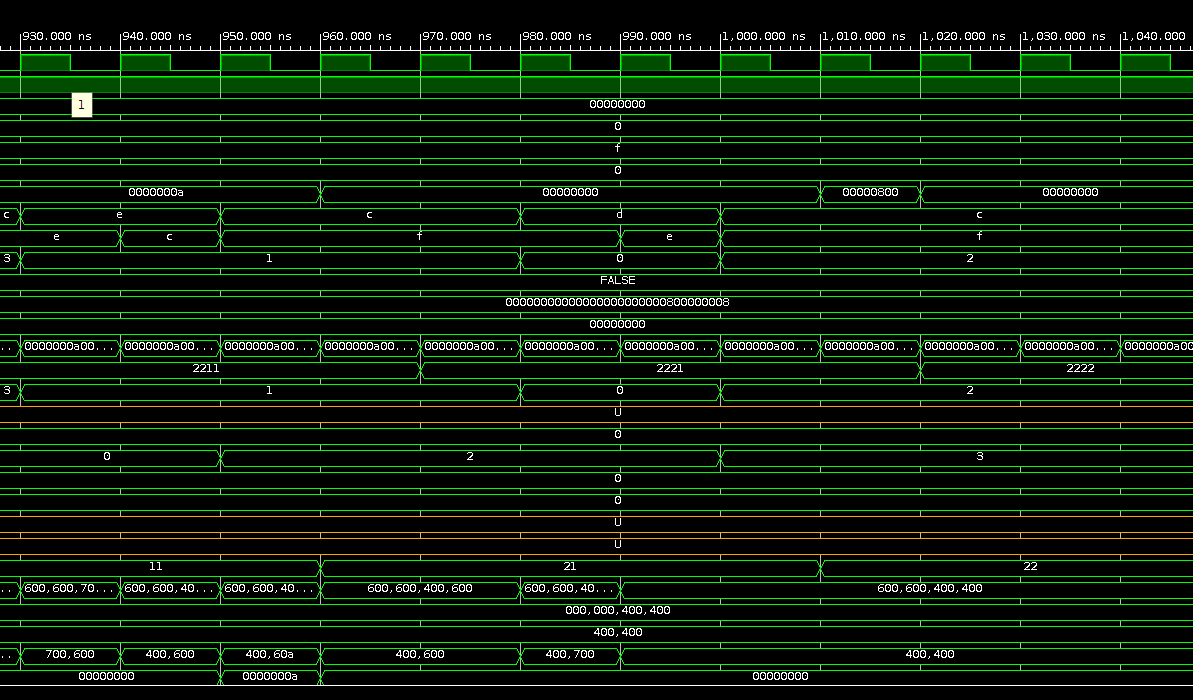
\includegraphics[width=.7\linewidth]{figures/new-sim/sim920.png}
	\caption{Simulation Result on 920}
	\label{fig:sim920}
\end{figure}

\newpage
960ns:    Data verified Server 1 send accept state set to ACTIVE 

970ns:    Client 1 set state to ACTIVE

1000ns:   Data verified Server 0 send accept state set to ACTIVE

1010ns:   Client 0 set state to ACTIVE
\begin{figure}[htb]
	\centering
	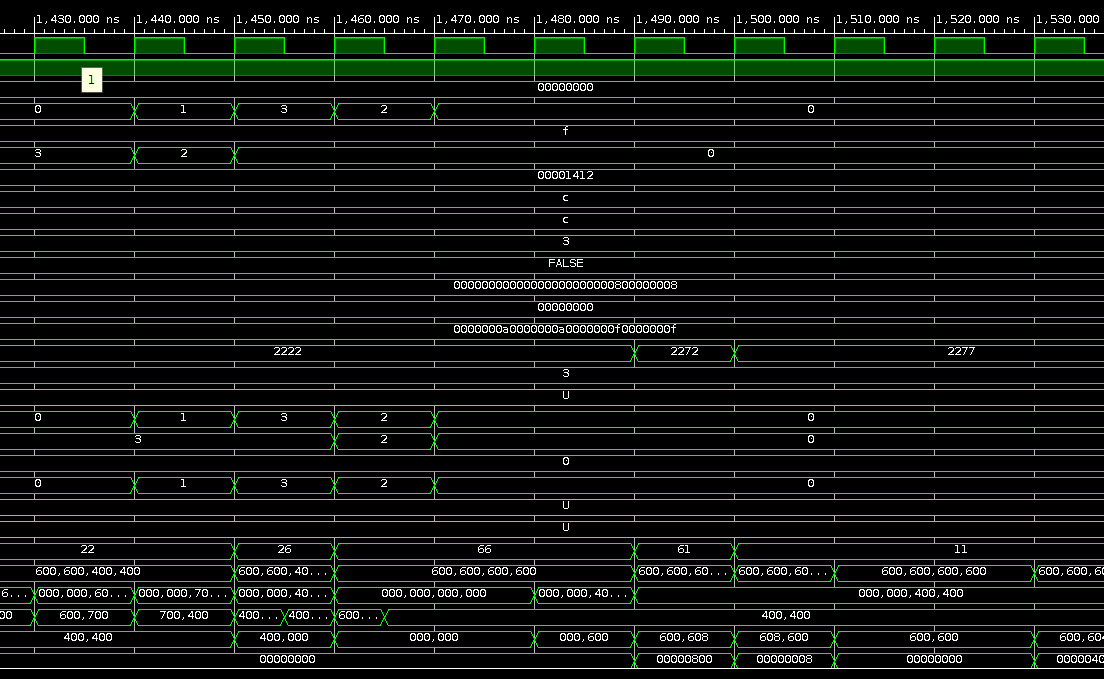
\includegraphics[width=.7\linewidth]{figures/new-sim/sim-1430.png}
	\caption{Simulation Result on 1430}
	\label{fig:sim1430}
\end{figure}

\newpage
1440ns:   Server 0 set state to SUCCEED

1450ns:   Server 1 set state to SUCCEED

1490ns:   Client 0 set state to 7, Server 1 set state to 1, 

1500ns:   Client 1 set state to 7, Server 0 set state to 1, 

1630ns:   Server 0 set state to ACTIVE 

1630ns:   Server 1 set state to ACTIVE 

2320ns:   Server 1 set state to SUCCEED, 

2350ns:   Server 0 set state to SUCCEED, 

\begin{figure}[htb]
	\centering
	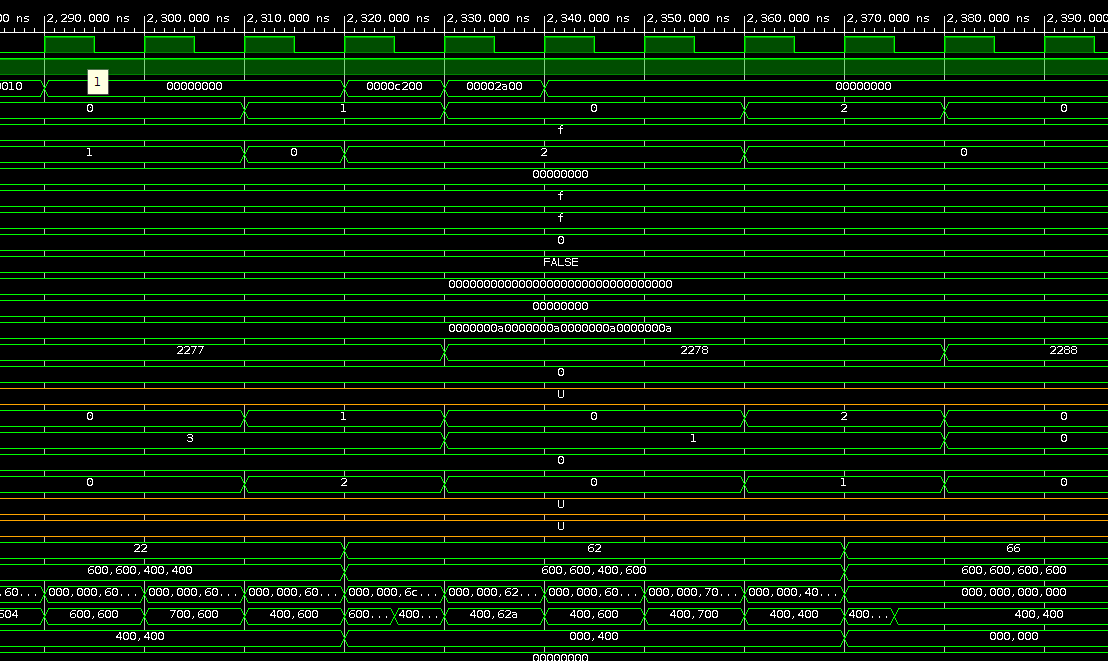
\includegraphics[width=.7\linewidth]{figures/new-sim/sim-2280.png}
	\caption{Simulation Result on 2280}
	\label{fig:sim2280}
\end{figure}


\section{Scaling Result}

This hardware architecture is designed to be easily scaled to fit different usage scenarios. Thanks to the VHDL generic mechanism, testing a architecture for more client nodes and server nodes requires changing the number in the generic part of the source code. 


\subsection{Flip-Flop Usage Scaling Result}

Flip-Flop is one of the most important resource in \gls{fpga} design to register data. Flip-Flop array is the core component of the priority table and atomic client/server register design. Flip-flops are also used in the client and server state-machine design to store their status. Scheduler policy implementations also have to use Flip-Flops, but the number is depend on its architecture and hard to predict. 

In this section, the usage of Flip-flop will be estimated first theoretically, then a software simulation in amd xilinx vivado\texttrademark will be posted to prove the conclusion.

\subsubsection{Priority Table }

Priority table is used to hold the priority number of all client nodes. The width of the priority number should be given by adjusting a parameter. This priority number width should be decided according to the specific scheduler policy. The FF usage is therefor linear to the number of clients if the priority number width is set.

Let F be the number of flip-flops, C the number of clients and W the width of a priority number.
     
$F = C \times W $

\subsubsection{Atomic Client Server Register}

The register has two parts, one for clients to hold the server that serving the client, one for servers to hold the client that the server is serving. Each client has also a bit to hold.

Let F be the number of flip-flops, C the number of clients S the number of servers and W the width of a priority number.
     
$F = C \times \log{S} + S \times \log{C} +C+S$

\subsubsection{Flip-Flop Usage Scaling on Client for 4 Servers}


Flip-Flop Usage Scaling on Client for 4 Servers, the more clients we have, the more Flip-Flop we need to add, the number scaled almost linearly 


\begin{table}[htb]
	\centering
	\caption{Flip-Flop Usage Scaling on Client for 4 Servers}
	\begin{tabular}{l c c}
		\toprule
		Server Number  & Client Number  & Flip-Flop\\ \midrule
        4	Servers	&	4	Clients	&	116	\\
        4	Servers	&	8	Clients	&	168	\\
        4	Servers	&	16	Clients	&	268	\\
        4	Servers	&	32	Clients	&	464	\\
        4	Servers	&	64	Clients	&	860	\\
        4	Servers	&	128	Clients	&	1642	\\
        4	Servers	&	256	Clients	&	3188	\\
		\bottomrule
	\end{tabular}
	\label{tab:ffs4}
\end{table}

 \begin{figure}[htb]
	\centering
	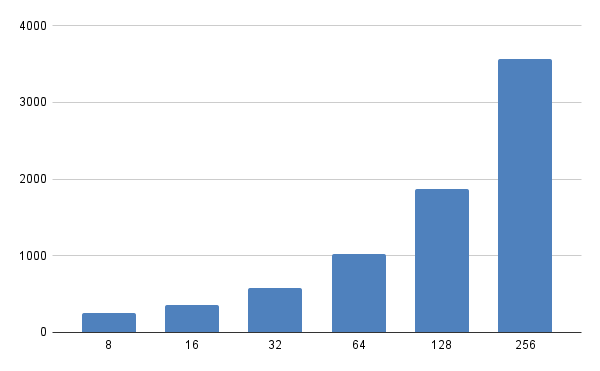
\includegraphics[width=.9\linewidth]{figures/Scaling/FF_4Server.png}
	\caption{Flip-Flop Usage Scaling on Client for 4 Servers}
	\label{fig:ffs4}
\end{figure}

\newpage


\subsubsection{Flip-Flop Usage Scaling on Client for 8 Servers}

\begin{table}[htb]
	\centering
	\caption{Flip-Flop Usage Scaling on Client for 8 Servers}
	\begin{tabular}{l c c}
		\toprule
		Server Number  & Client Number  & Flip-Flop\\ \midrule
        8	Servers	&	8	Clients	&	248	\\
        8	Servers	&	16	Clients	&	360	\\
        8	Servers	&	32	Clients	&	576	\\
        8	Servers	&	64	Clients	&	1016	\\
        8	Servers	&	128	Clients	&	1872	\\
        8	Servers	&	256	Clients	&	3560	\\
		\bottomrule
	\end{tabular}
	\label{tab:FF-8Server}
\end{table}

 \begin{figure}[h]
	\centering
	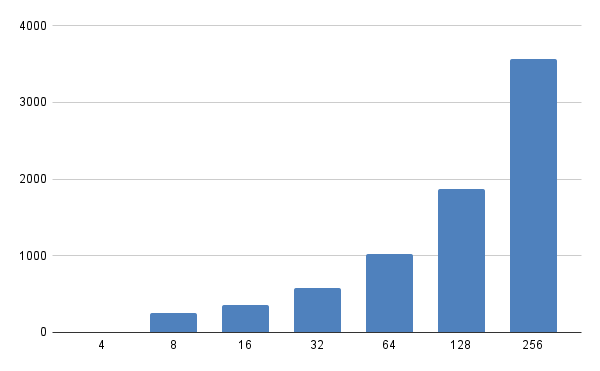
\includegraphics[width=.9\linewidth]{figures/Scaling/FF-8Server.png}
	\caption{Flip-Flop Usage Scaling on Client for 8 Servers}
	\label{fig:ffs8}
\end{figure}

Flip-Flop Usage Scaling on Client for 8 Servers, the usage almost doubled as the Flip-Flop usage than the last simulation.

In this scenario, the Flip-Flop also scaled almost linearly. 
\newpage
\subsubsection{Flip-Flop Usage Scaling on Client for 256 Servers}

\begin{table}[htb]
	\centering
	\caption{Flip-Flop Usage Scaling on Client for 256 Servers}
	\begin{tabular}{l c c}
		\toprule
		Server Number  & Client Number  & Flip-Flop\\ \midrule
        256	Servers	&	8	Clients	&	5016	\\
        256	Servers	&	16	Clients	&	5680	\\
        256	Servers	&	32	Clients	&	6752	\\
        256	Servers	&	64	Clients	&	9152	\\
		\bottomrule
	\end{tabular}
	\label{tab:FF-256S}
\end{table}

\begin{figure}[h]
	\centering
	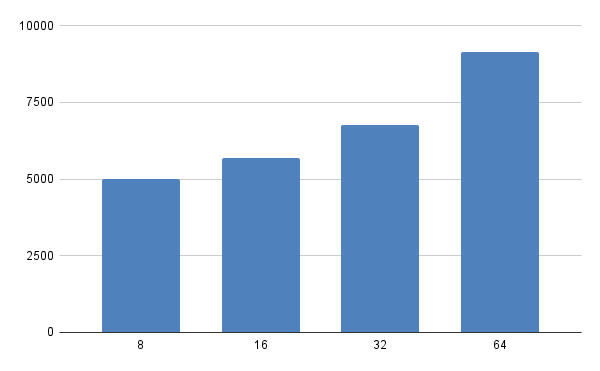
\includegraphics[width=.9\linewidth]{figures/Scaling/FF-256S.png}
	\caption{Flip-Flop Usage Scaling on Client for 256 Servers}
	\label{fig:ffs256}
\end{figure}

We change the Server number to 256 this time and the resource usage is huge. user should avoid that large number of client and server combination and choose a better topology of nodes. 
\newpage
\subsubsection{Flip-Flop Usage Scaling on Servers for 8 Clients}

\begin{table}[htb]
	\centering
	\caption{Flip-Flop Usage Scaling on Server for 8 Clients}
	\begin{tabular}{l c c}
		\toprule
    	Client Number  & Server Number  & Flip-Flop\\ \midrule
        8	Clients	&	2	Servers	&	124	\\
        8	Clients	&	4	Servers	&	168	\\
        8	Clients	&	8	Servers	&	248	\\
        8	Clients	&	16	Servers	&	400	\\
        8	Clients	&	32	Servers	&	693	\\
        8	Clients	&	64	Servers	&	1303	\\
        8	Clients	&	128	Servers	&	2504	\\
        8	Clients	&	256	Servers	&	5016	\\
		\bottomrule
	\end{tabular}
	\label{tab:ffc8}
\end{table}

\begin{figure}[h]
	\centering
	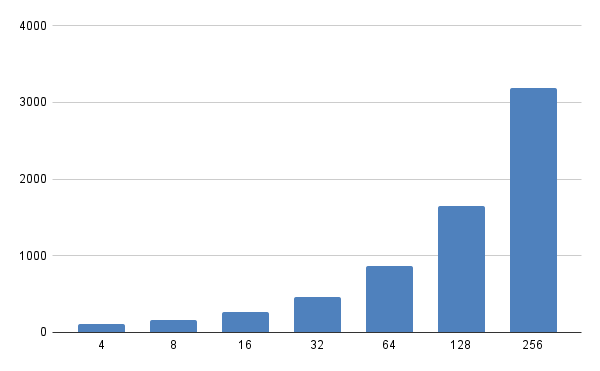
\includegraphics[width=.9\linewidth]{figures/Scaling/FF-8Client.png}
	\caption{Flip-Flop Usage Scaling on Server for 8 Clients}
	\label{fig:ffc8}
\end{figure}

This time we fixed the number of client and see how Flip-Flop usage scales on server number. The result is the same, resources usage grows linearly as number of server rises.

\newpage
\subsection{Lookup Table Usage Scaling Result}

Lookup Table Usage Scaling on Client for 4 Servers, the more clients we have, the more Lookup Table Usage we need to add, the number scaled almost linearly therefor we know, do not use that big numbers or you will use up all the FPGA resources and have a low overhead code percentage.

\subsubsection{Lookup Table Usage Scaling on Clients for 4 Servers}

\begin{table}[htb]
	\centering
	\caption{Lookup Table Usage Scaling on Clients for 4 Servers}
	\begin{tabular}{l c c}
		\toprule
    	Client Number  & Server Number  & Lookup Table\\ \midrule
        4	Clients	&	4	Servers	&	405	\\
        8	Clients	&	4	Servers	&	742	\\
        16	Clients	&	4	Servers	&	1341	\\
        32	Clients	&	4	Servers	&	2374	\\
        64	Clients	&	4	Servers	&	4822	\\
        128	Clients	&	4	Servers	&	9333	\\
        256	Clients	&	4	Servers	&	18857	\\
		\bottomrule
	\end{tabular}
	\label{tab:luts4}
\end{table}

 \begin{figure}[h]
	\centering
	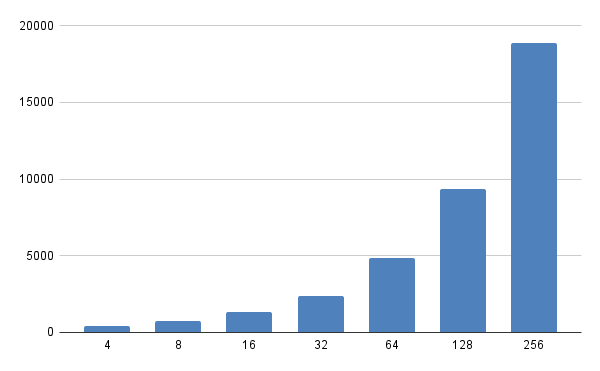
\includegraphics[width=.9\linewidth]{figures/Scaling/LUT4.png}
	\caption{Lookup Table Usage Scaling on Client for 4 Servers}
	\label{fig:luts4}
\end{figure}
\newpage
\subsubsection{Lookup Table Usage Scaling on Clients for 8 Servers}

Lookup Table Usage Scaling on Client for 8 Servers, the usage almost doubled as the Lookup Table usage than the last simulation.

In this scenario, the Flip-Flop also scaled almost linearly. 

\begin{table}[htb]
	\centering
	\caption{Lookup Table Usage Scaling on Clients for 8 Servers}
	\begin{tabular}{l c c}
		\toprule
    	Client Number  & Server Number  & Lookup Table\\ \midrule
        8	Clients	&	8	Servers	&	1143	\\
        16	Clients	&	8	Servers	&	2044	\\
        32	Clients	&	8	Servers	&	3709	\\
        64	Clients	&	8	Servers	&	7342	\\
        128	Clients	&	8	Servers	&	14314	\\
        256	Clients	&	8	Servers	&	28542	\\
		\bottomrule
	\end{tabular}
	\label{tab:luts8}
\end{table}

 \begin{figure}[h]
	\centering
	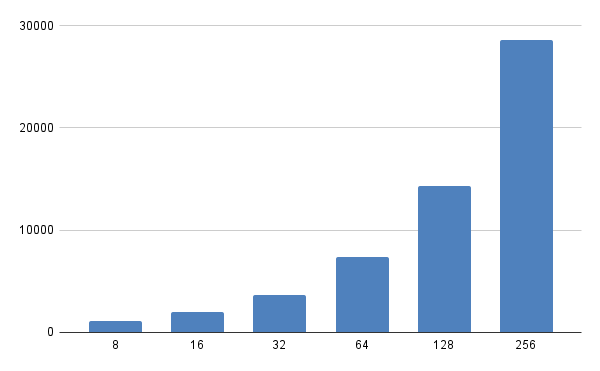
\includegraphics[width=.7\linewidth]{figures/Scaling/LUTS8.png}
	\caption{Lookup Table Usage Scaling on Client for 8 Servers}
	\label{fig:luts8}
\end{figure}

\newpage
\subsubsection{Lookup Table Usage Scaling on Clients for 256 Servers}

We change the Server number to 256 this time and the resource usage is huge also for lookup tables. User should avoid that large number of client and server combination and choose a better topology of nodes. 

\begin{table}[htb]
	\centering
	\caption{Lookup Table Usage Scaling on Clients for 256 Servers}
	\begin{tabular}{l c c}
		\toprule
    	Client Number  & Server Number  & Lookup Table\\ \midrule
        8	Clients	&	8	Servers	&	25032	\\
        16	Clients	&	8	Servers	&	39965	\\
        32	Clients	&	8	Servers	&	70665	\\
        64	Clients	&	8	Servers	&	134825	\\
		\bottomrule
	\end{tabular}
	\label{tab:lut256s}
\end{table}

\begin{figure}[h]
	\centering
	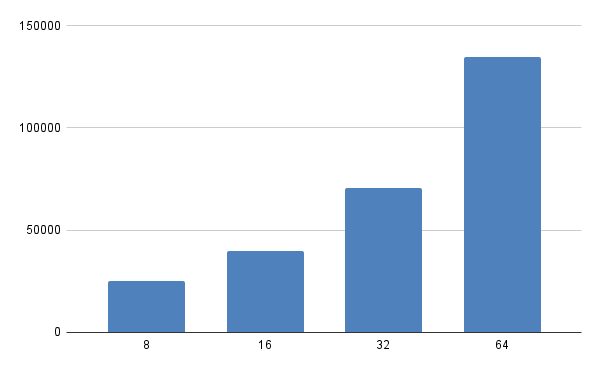
\includegraphics[width=.9\linewidth]{figures/Scaling/LUTS256.png}
	\caption{Lookup Table Usage Scaling on Client for 256 Servers}
	\label{fig:luts256}
\end{figure}
\newpage
\subsubsection{Lookup Table Usage Scaling on Servers for 8 Clients}

This time we fixed the number of client and see how Lookup Table usage scales on server number. The result is the same, resources usage grows linearly as number of server rises.

\begin{table}[htb]
	\centering
	\caption{Lookup Table Usage Scaling on Servers for 8 Clients}
	\begin{tabular}{l c c}
		\toprule
    	Server Number  & Client Number  & Lookup Table\\ \midrule
        2	Servers	&	8	Clients	&	594	\\
        4	Servers	&	8	Clients	&	742	\\
        8	Servers	&	8	Clients	&	1143	\\
        16	Servers	&	8	Clients	&	1871	\\
        32	Servers	&	8	Clients	&	3310	\\
        64	Servers	&	8	Clients	&	6321	\\
        128	Servers	&	8	Clients	&	12686	\\
        256	Servers	&	8	Clients	&	25032	\\
		\bottomrule
	\end{tabular}
	\label{tab:lutc8}
\end{table}

\begin{figure}[h]
	\centering
	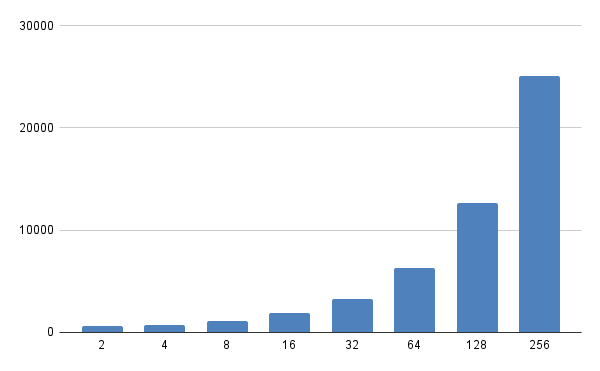
\includegraphics[width=.9\linewidth]{figures/Scaling/LUTC8.png}
	\caption{Lookup Table Usage Scaling on Server for 8 Clients}
	\label{fig:lutc8}
\end{figure}
